\documentclass[a4paper, 12pt, twoside, openright]{book}

% -------------------------------------------------------------------------
% GENERAL NOTES
% To compile this file, you need to have at least one citation and one defined acronym
% Define one citation in 'Sections/reference_list.bib' and use any of the \cite commands anywhere in the text to avoid errors
% Define one acronym in 'Sections/4.5-list_of_acronyms.tex' and use \an{defined-acronym} anywhere in the text to avoid errors
% -------------------------------------------------------------------------

% Configurations for the TeX template
% !TeX root = ..\Thesis.tex

% Encoding and Language
\usepackage[utf8]{inputenc}  % Input encoding, allows the use of UTF-8 characters
\usepackage[portuguese]{babel}  % Language support, here set to English
\usepackage[T1]{fontenc}     % Output font encoding, improves handling of special characters

% Mathematics
\usepackage{amsmath, amssymb}   % Basic math symbols and environments
\usepackage{dsfont}             % Double-struck fonts (e.g., for the indicator function)
\usepackage{bm}                 % Bold math symbols
\usepackage{mathrsfs}           % Additional math script fonts

% Graphics and Figures
\usepackage{graphicx}           % Include images and graphics
\usepackage{float}              % Improved control over float placement
%\floatstyle{boxed}             % Option for boxed floats (currently commented out)
\restylefloat{figure}           % Allows restyling of figure floats
\usepackage{subcaption}         % Sub-figures within a single figure
\usepackage[font={footnotesize,it}]{caption}  % Caption formatting, small and italic
\usepackage{adjustbox}          % Adjust size and alignment of content (e.g., images)


% Tables
% https://people.inf.ethz.ch/markusp/teaching/guides/guide-tables.pdf
\usepackage{booktabs}           % Professional-quality tables
\usepackage{threeparttable}     % Tables with notes below them
\usepackage{makecell}           % Customizable cell format in tables
\usepackage{multicol, multirow} % Multi-column and multi-row cells in tables
\usepackage[table]{xcolor}      % Color support in tables (and elsewhere)

% Text Formatting and Styling
\usepackage{color}              % Colored text
\usepackage{url}                % Proper formatting of URLs
\usepackage{fancyhdr}           % Custom headers and footers
\usepackage[procnames]{listings} % Code listings with syntax highlighting
\usepackage{lstautogobble}      % To remove empty lines at the end of listing envs
\usepackage[onehalfspacing]{setspace}  % Line spacing adjustments (1.5 spacing here)
\usepackage[nottoc]{tocbibind}  % Add bibliography/index to the Table of Contents

% Float Management
\usepackage{flafter}            % Prevents floats from appearing before their references
\usepackage[section]{placeins}  % Prevents floats from leaving their section

% Layout and Geometry
\usepackage[a4paper, left=3cm, right=2cm, top=3cm, bottom=2cm]{geometry}  % Page margins
\usepackage[space]{grffile}     % Allows spaces in graphic file names
%\usepackage{showframe}         % Displays the layout frames (currently commented out)
%\usepackage{fullpage}          % Use full page layout (currently commented out)
%\usepackage{comment}           % Allows commenting out large sections of text

% Special Features
\usepackage{eso-pic}            % Add background picture to pages (e.g., title page)
\usepackage{natbib}             % Bibliography and citations with NatBib
\usepackage{acro}               % Enables the definition and management of acronyms
\usepackage{tcolorbox}          % For bounding boxes
\usepackage{siunitx}            % Physical units
%\usepackage[printonlyused, withpage]{acronym} % Enables the definition and management of acronyms (another way)
%\usepackage{icomma}            % Adjust spacing after commas in math mode (currently commented out)
%\usepackage{array}             % Advanced table options (currently commented out)
%\setlength{\extrarowheight}{.5ex}  % Extra row height for tables (use with array package)
%\usepackage[outline]{contour}  % Outlined text (currently commented out)
\usepackage{layouts} 
\usepackage{tikz}
\usetikzlibrary{shapes, arrows.meta, positioning, shapes.geometric, fit}

\usepackage[indent=1.5cm]{parskip} % 1.5cm identation, following ABNT rules

% \newcommand{\ra}[1]{\renewcommand{\arraystretch}{#1}}  % Adjusts row spacing in tables

% ------------------------------------------------------------------------------
% Optional Packages
% ------------------------------------------------------------------------------
% Uncomment if you want to use these features

% Minted: Code listings with syntax highlighting
%\usepackage{minted}
%\usemintedstyle{pastie}  % Pastie style for minted code blocks

% Line Numbers
\usepackage{lineno}
% \linenumbers  % Enables line numbering, comment this line to remove them

% ------------------------------------------------------------------------------
% Define dynamic chapter titles based on language
% ------------------------------------------------------------------------------
\providecommand{\chapternameintro}{%
  \iflanguage{portuguese}{Introdução}{Introduction}}
\providecommand{\chapternamedatabase}{%
  \iflanguage{portuguese}{Base de dados fotométricos}{Data base}}
\providecommand{\chapternameanalysis}{%
  \iflanguage{portuguese}{UCDs na região de Fornax}{Analysis}}
\providecommand{\chapternamespectra}{%
  \iflanguage{portuguese}{Espectroscopia de uma amostra de candidatas a UCDs em Fornax}{Spectra}}
\providecommand{\chapternamespectraemission}{%
  \iflanguage{portuguese}{Objetos compactos com emissão}{Compact objects with emission lines}}
\providecommand{\chapternameconclusions}{%
  \iflanguage{portuguese}{Conclusões}{Conclusions}}
\providecommand{\chapternamefuture}{%
  \iflanguage{portuguese}{Perspectivas futuras}{Future perspectives}}
\providecommand{\chapternameacronyms}{%
  \iflanguage{portuguese}{Lista de Acrônimos}{List of Acronyms}}
\providecommand{\chapternameappendix}{%
  \iflanguage{portuguese}{Observações de candidatas a UCDs com o Gemini Sul}{Appendix}}

% ------------------------------------------------------------------------------
% Listing theme
% ------------------------------------------------------------------------------
% https://tex.stackexchange.com/questions/235731/listings-syntax-for-literate

\definecolor{codegreen}{rgb}{0,0.6,0}
\definecolor{codegray}{rgb}{0.5,0.5,0.5}
\definecolor{codepurple}{rgb}{0.58,0,0.82}
\definecolor{backcolour}{rgb}{0.97,0.97,0.97}
 
\lstdefinestyle{mystyle}{
    morekeywords={access,and,break,class,continue,def,del,elif,else,except,exec,
    finally,for,from,global,if,import,in,is,lambda,not,or,pass,print,raise,
    return,self,try,while},
    morekeywords=[2]{abs,all,any,basestring,bin,bool,bytearray,callable,chr,
    classmethod,cmp,compile,complex,delattr,dict,dir,divmod,enumerate,eval,
    execfile,file,filter,float,format,frozenset,getattr,globals,hasattr,hash,
    help,hex,id,input,int,isinstance,issubclass,iter,len,list,locals,long,map,
    max,memoryview,min,next,object,oct,open,ord,pow,property,range,raw_input,
    reduce,reload,repr,reversed,round,set,setattr,slice,sorted,staticmethod,str,
    sum,super,tuple,type,unichr,unicode,vars,xrange,zip,apply,buffer,coerce,
    intern},
    backgroundcolor=\color{backcolour},
    commentstyle=\color{codegreen},
    keywordstyle=\color{magenta},
    numberstyle=\tiny\color{codegray},
    stringstyle=\color{codepurple},
    basicstyle=\scriptsize\ttfamily,
    breakatwhitespace=false,
    breaklines=true,
    captionpos=b,
    keepspaces=true,
    numbers=left,
    numbersep=10pt,
    showspaces=false,
    showstringspaces=false,
    showtabs=false,
    tabsize=2,
    frame=single,
    frameround={t}{t}{t}{t},
    framexleftmargin=6mm,
    xleftmargin=20pt,
    xrightmargin=3pt
    }
\lstset{style=mystyle}

% ------------------------------------------------------------------------------
% Custom Page Elements and Layout Adjustments
% ------------------------------------------------------------------------------

% Create a new environment that defines a right-aligned box
\newenvironment{rightbox}[1]
 {\itemize[
    nosep,
    leftmargin=\dimexpr\textwidth-#1\relax,
    rightmargin=0pt,
    itemindent=\parindent,
    listparindent=\parindent,
  ]\item[]\relax}
 {\enditemize}

% Command to create a blank page
\newcommand\blankpage{%
    \null
    \thispagestyle{empty}%
    \addtocounter{page}{-1}%
    \newpage
}

% Fancy Header Configuration
\fancyhead{}  % Clear default header
\fancyfoot{}  % Clear default footer
\fancyhead[RO,LE]{\thepage}  % Page number on the right for odd pages and left for even pages
\fancyhead[CE]{\nouppercase\leftmark}  % Section title centered on even pages
\fancyhead[CO]{\nouppercase\rightmark} % Chapter title centered on odd pages
\pagestyle{fancy}  % Apply fancyhdr configuration

% Customization of section marks in headers
\renewcommand{\sectionmark}[1]{%
    \markright{\scriptsize{\slshape{\fontsize{10}{12} \selectfont Section \thesection.\ #1}}}
}
\renewcommand{\headrulewidth}{0.7pt}  % Line width for header rule
\setlength{\headheight}{14pt}  % Adjust header height

% ------------------------------------------------------------------------------
% Custom Commands for Color
% ------------------------------------------------------------------------------

\definecolor{lightgray}{gray}{0.7}  % Define light gray color
\definecolor{gray75}{gray}{0.75}  % Define 75% gray color

% ------------------------------------------------------------------------------
% Page Layout and Section Formatting
% ------------------------------------------------------------------------------

\usepackage{emptypage}  % Suppresses page numbers on empty pages
\usepackage{titlesec, blindtext}  % Customization of section titles

% Customization of the Table of Contents
\renewcommand\contentsname{Table of Contents}
\titleformat{\chapter}[display]  % Format for chapters with number
{\bfseries\Huge}
{{\chaptertitlename} \large\thechapter}
{2ex}
{\titlerule\vspace{2ex}}

\titleformat{name=\chapter,numberless}[display]  % Format for unnumbered chapters
{\bfseries\Huge}
{\color{gray75}{\titlerule[0.8pt]}}
{-8ex} % Should be -7ex if not using parskip
{\bfseries\Huge}[]

% Customizing how chapters, sections, and subsections are displayed
\titleformat{\chapter}[hang]{\Huge\bfseries}  % Chapter format
{\thechapter\hsp\textcolor{gray75}{}\hsp}{0pt}{\Huge\bfseries}
[\color{gray75}{\titlerule[.8pt]}]

\titleformat{\section}[hang]{\LARGE\bfseries}  % Section format
{\thesection\hspace{19pt}\textcolor{gray75}{|}\hspace{14pt}}{0pt}{\LARGE\bfseries}
[]

\titleformat{\subsection}[hang]{\Large\bfseries}  % Subsection format
{\makebox[1cm]{\thesubsection}\hsp\textcolor{gray75}{|}\hsp}{0pt}{\Large\bfseries}
[]

% Adjust spacing around titles
% \titlespacing{command%plain}{left%l}{before-sep%l}{after-sep%l}
\titlespacing{\chapter}{0pt}{0pt}{1.0cm}
\titlespacing{\section}{0pt}{1.0cm}{1.0cm}
\titlespacing{\subsection}{0pt}{1.0cm}{1.0cm}
\titlespacing{\subsubsection}{0pt}{1.0cm}{1.0cm}

% Add numbering to subsubsections
\setcounter{secnumdepth}{3}

% ------------------------------------------------------------------------------
% Background Image on First Page (uncomment if you want the USP symbol in
% the first page)
% ------------------------------------------------------------------------------

% \newcommand\BackgroundPic{%
%     \put(0,0){%
%         \parbox[b][\paperheight]{\paperwidth}{%
%             \vfill
%             \centering
%             
\includegraphics[width=.9\paperwidth,height=.9\paperheight,%
%                 keepaspectratio]{Images/brasao_usp_pb_c}%
%             \vfill
%         }}
% }

% ------------------------------------------------------------------------------
% Acronym Management
% ------------------------------------------------------------------------------

\acsetup{
  single         = true,
  list/sort      = true,
  cite/display   = first,
  cite/group     = true,
  cite/cmd       = \citep,
  cite/group/cmd = \citealp
}

% Reset acronyms each chapter (so LaTeX shows the long name again)
\preto\chapter\acresetall

% ------------------------------------------------------------------------------
% Hyperlinks and References
% ------------------------------------------------------------------------------

\usepackage{hyperref}  % Should be loaded last
\hypersetup{
    colorlinks,
    linkcolor=blue,
    anchorcolor=blue,
    citecolor=blue,
    filecolor=blue,
    menucolor=blue,
    runcolor=blue,
    urlcolor=blue,
}

% ------------------------------------------------------------------------------
% Additional Customizations
% ------------------------------------------------------------------------------

% ABNT style for itemized lists using a dash
\def\labelitemi{\normalfont\bfseries \textendash}  

% Adjust float placement separation
\makeatletter
\setlength{\@fpsep}{1cm}  % Adjust value as needed
\makeatother

% Ensure subsections behave correctly
\makeatletter
\AtBeginDocument{%
    \expandafter\renewcommand\expandafter\subsection\expandafter{%
        \expandafter\@fb@secFB\subsection
    }%
}
\makeatother

% Custom command to manually number equations
\newcommand\numberthis{\addtocounter{equation}{1}\tag{\theequation}}

% Adjust fraction of text on a page
\def\textfraction{0.1}

% Set the path for images
\graphicspath{{Images/}}

% Defining acronyms
% Warning: this code will give an error if you define acronyms but not use any in the text (this happens e.g. you are starting a new document)

\DeclareAcronym{splus}{
  short = S-PLUS,
  long  = Southern Photometric Local Universe Survey,
  cite  = oliveira2019splus
}

\DeclareAcronym{sdss}{
  short = SDSS,
  long  = Sloan Digital Sky Survey,
  cite  = york2000sdss
}

\DeclareAcronym{galex}{
  short = GALEX,
  long  = Galaxy Evolution Explorer,
  cite  = martin2005galex
}

\DeclareAcronym{vhs}{
  short = VHS,
  long  = Vista Hemisphere Survey,
  cite  = mcmahon2013vhs
}

\DeclareAcronym{des}{
  short = DES,
  long  = Dark Energy Survey,
  cite  = sanchez2010des
}

\DeclareAcronym{lsst}{
  short = LSST,
  long  = Legacy Survey of Space and Time,
  cite  = ivezic2008lsst
}

\DeclareAcronym{lss}{
  short = LSS,
  long  = large-scale structure
}

\DeclareAcronym{photoz}{
  short = photo-$z$,
  long  = redshifts fotométricos
}

\DeclareAcronym{specz}{
  short = spec-$z$,
  long  = redshifts espectroscópicos
}

\DeclareAcronym{UCD}{
  short = UCDs,
  long  = Galáxias Anã Ultra-Compactas (Ultra-Compact Dwarf galaxies)
}

\DeclareAcronym{GC}{
  short = GC,
  long  = Aglomerados Globularess
}

\DeclareAcronym{NSC}{
  short = NSC,
  long  = Núcleo Estelar
}

\DeclareAcronym{DR4}{
  short = DR4,
  long  = Data Release 4
}

\DeclareAcronym{RA}{
  short = RA,
  long  = Ascensão Reta
}

\DeclareAcronym{DEC}{
  short = DEC,
  long  = Declinação
}

\DeclareAcronym{FWHM}{
  short = FWHM,
  long  = Largura a Meia Altura
}

\DeclareAcronym{GMOS-S}{
  short = GMOS-S,
  long  = Gemini Multi-Object Spectrograph South
}

\DeclareAcronym{PM}{
  short = PM,
  long  = Movimento Próprio
}

\DeclareAcronym{CMD}{
  short = CMD,
  long  = Diagrama Cor-Magnitude
}

\DeclareAcronym{ML}{
  short = ML,
  long  = Aprendizado de Máquina
}

\DeclareAcronym{RF}{
  short = RF,
  long  = Random Forest
}

\DeclareAcronym{KNN}{
  short = KNN,
  long  = K-Nearest Neighbors
}

\DeclareAcronym{SExtractor}{
  short = SExtractor,
  long  = Source Extractor
}

\DeclareAcronym{BCD}{
  short = BCD,
  long  = Galáxias anãs azuis
}

\DeclareAcronym{dSph}{
  short = dSph,
  long  = galáxias anãs esferoidais
}

\DeclareAcronym{dE}{
  short = dE,
  long  = anãs elípticas
}

\DeclareAcronym{dIrr}{
  short = dIrr,
  long  = dwarf Irregular galaxy
}

\DeclareAcronym{UDG}{
  short = UDG,
  long  = galáxias anãs ultradifusas
}
% To use acronyms, use \an{defined-acronym} in the text.

% ----------------------------------------------------------------------------------------------------------------------
% Defining custom commands
\newcommand{\red}[1]{\textbf{\textcolor{red}{#1}}}  % Command for red text
\newcommand{\hsp}{\hspace{15pt}}  % Command for horizontal space
\renewcommand{\geq}{\geqslant}  % Redefine >= symbol
\renewcommand{\leq}{\leqslant}  % Redefine <= symbol
\newcommand{\ttt}[1]{\texttt{#1}} % Alias for \texttt
\DeclareSIUnit{\angstrom}{\textup{\AA}} % Angstrom unit, to be used with the siunitx package
\newcommand{\ionn}[2]{{\textrm{#1}}{\textrm{\sc #2}}} % Commando to print ions, for ex. [\ionn{O}{ii}]
\newcommand{\review}[1]{\textbf{\textcolor{orange}{#1}}}
\DeclareMathOperator*{\aprox}{\approx}  % Custom operator for 'approximately equal'

% ----------------------------------------------------------------------------------------------------------------------
% Configurations
\newcommand{\authorname}{Seu nome} % Author name
\newcommand{\supervisorname}{Prof. Dr. Nome do Orientador} % Supervisor name
\newcommand{\thesistitle}{Template não oficial para dissertações e teses do IAG-USP} % Thesis title

% ----------------------------------------------------------------------------------------------------------------------
% Document body
\begin{document}
%\pagevalues
\onehalfspacing

% Journal macros (for references)
% Ref macros
\let\jnl@\rm
\def\refs@jnl#1{{\rm#1}}

\def\aj{\refs@jnl{AJ}}                   % Astronomical Journal
\def\actaa{\refs@jnl{Acta Astron.}}      % Acta Astronomica
\def\araa{\refs@jnl{ARA\&A}}             % Annual Review of Astron and Astrophys
\def\apj{\refs@jnl{ApJ}}                 % Astrophysical Journal
\def\apjl{\refs@jnl{ApJ}}                % Astrophysical Journal, Letters
\def\apjs{\refs@jnl{ApJS}}               % Astrophysical Journal, Supplement
\def\asr{\refs@njl{Adv. Space Res.}}     % Advances in Space Research
\def\ao{\refs@jnl{Appl.~Opt.}}           % Applied Optics
\def\apss{\refs@jnl{Ap\&SS}}             % Astrophysics and Space Science
\def\ag{\refs@njl{Astron. Geophys.}}     % Astronomy and Geophysics
\def\aap{\refs@jnl{A\&A}}                % Astronomy and Astrophysics
\def\aapr{\refs@jnl{A\&A~Rev.}}          % Astronomy and Astrophysics Reviews
\def\aaps{\refs@jnl{A\&AS}}              % Astronomy and Astrophysics, Supplement
\def\azh{\refs@jnl{AZh}}                 % Astronomicheskii Zhurnal
\def\baas{\refs@jnl{BAAS}}               % Bulletin of the AAS
\def\bac{\refs@jnl{Bull. astr. Inst. Czechosl.}}
                % Bulletin of the Astronomical Institutes of Czechoslovakia 
\def\caa{\refs@jnl{Chinese Astron. Astrophys.}}
                % Chinese Astronomy and Astrophysics
\def\cjaa{\refs@jnl{Chinese J. Astron. Astrophys.}}
                % Chinese Journal of Astronomy and Astrophysics
\def\icarus{\refs@jnl{Icarus}}           % Icarus
\def\jcap{\refs@jnl{J. Cosmology Astropart. Phys.}}
                % Journal of Cosmology and Astroparticle Physics
\def\jrasc{\refs@jnl{JRASC}}             % Journal of the RAS of Canada
\def\memras{\refs@jnl{MmRAS}}            % Memoirs of the RAS
\def\mnras{\refs@jnl{MNRAS}}             % Monthly Notices of the RAS
\def\na{\refs@jnl{New A}}                % New Astronomy
\def\nar{\refs@jnl{New A Rev.}}          % New Astronomy Review
\def\pra{\refs@jnl{Phys.~Rev.~A}}        % Physical Review A: General Physics
\def\prb{\refs@jnl{Phys.~Rev.~B}}        % Physical Review B: Solid State
\def\prc{\refs@jnl{Phys.~Rev.~C}}        % Physical Review C
\def\prd{\refs@jnl{Phys.~Rev.~D}}        % Physical Review D
\def\pre{\refs@jnl{Phys.~Rev.~E}}        % Physical Review E
\def\prl{\refs@jnl{Phys.~Rev.~Lett.}}    % Physical Review Letters
\def\pasa{\refs@jnl{PASA}}               % Publications of the Astron. Soc. of Australia
\def\pasp{\refs@jnl{PASP}}               % Publications of the ASP
\def\pasj{\refs@jnl{PASJ}}               % Publications of the ASJ
\def\rmxaa{\refs@jnl{Rev. Mexicana Astron. Astrofis.}}%
                % Revista Mexicana de Astronomia y Astrofisica
\def\qjras{\refs@jnl{QJRAS}}             % Quarterly Journal of the RAS
\def\skytel{\refs@jnl{S\&T}}             % Sky and Telescope
\def\solphys{\refs@jnl{Sol.~Phys.}}      % Solar Physics
\def\sovast{\refs@jnl{Soviet~Ast.}}      % Soviet Astronomy
\def\ssr{\refs@jnl{Space~Sci.~Rev.}}     % Space Science Reviews
\def\zap{\refs@jnl{ZAp}}                 % Zeitschrift fuer Astrophysik
\def\nat{\refs@jnl{Nature}}              % Nature
\def\iaucirc{\refs@jnl{IAU~Circ.}}       % IAU Cirulars
\def\aplett{\refs@jnl{Astrophys.~Lett.}} % Astrophysics Letters
\def\apspr{\refs@jnl{Astrophys.~Space~Phys.~Res.}}
                % Astrophysics Space Physics Research
\def\bain{\refs@jnl{Bull.~Astron.~Inst.~Netherlands}} 
                % Bulletin Astronomical Institute of the Netherlands
\def\fcp{\refs@jnl{Fund.~Cosmic~Phys.}}  % Fundamental Cosmic Physics
\def\gca{\refs@jnl{Geochim.~Cosmochim.~Acta}}   % Geochimica Cosmochimica Acta
\def\grl{\refs@jnl{Geophys.~Res.~Lett.}} % Geophysics Research Letters
\def\jcp{\refs@jnl{J.~Chem.~Phys.}}      % Journal of Chemical Physics
\def\jgr{\refs@jnl{J.~Geophys.~Res.}}    % Journal of Geophysics Research
\def\jqsrt{\refs@jnl{J.~Quant.~Spec.~Radiat.~Transf.}}
                % Journal of Quantitiative Spectroscopy and Radiative Transfer
\def\memsai{\refs@jnl{Mem.~Soc.~Astron.~Italiana}}
                % Mem. Societa Astronomica Italiana
\def\nphysa{\refs@jnl{Nucl.~Phys.~A}}   % Nuclear Physics A
\def\physrep{\refs@jnl{Phys.~Rep.}}   % Physics Reports
\def\physscr{\refs@jnl{Phys.~Scr}}   % Physica Scripta
\def\planss{\refs@jnl{Planet.~Space~Sci.}}   % Planetary Space Science
\def\procspie{\refs@jnl{Proc.~SPIE}}   % Proceedings of the SPIE

\let\astap=\aap
\let\apjlett=\apjl
\let\apjsupp=\apjs
\let\applopt=\ao

\newpage

% Starting pages
% Title page, signature page, 'original' or 'corrected' version page
%%%%%%%%%%%%%%%%%%%%%%%%%%%%%%%%%%%%%%%%%%%%%%%% Title page
%\newgeometry{centering}    %%% make the page centered on paper
\newgeometry{left=3.5cm, right=3.5cm, bottom=2cm}

%\AddToShipoutPicture*{\BackgroundPic}
\thispagestyle{empty}%\addtocounter{page}{-1}
\begin{center}
  \Large{
    Universidade de São Paulo \\
    Instituto de Astronomia, Geofísica e Ciências Atmosféricas \\
    Departamento de Astronomia
  }
  
  \vspace*{3cm}

  \LARGE{\authorname}

  \vspace{3cm}

  \begin{center}
    \begin{huge}
      \textbf{\thesistitle}
    \end{huge}
  \end{center}

  \vfill

  \Large{
    São Paulo \\
    \the\year\\
  }
\end{center}

\newpage
\shipout\null %Comando para adicionar uma página em branco 

%%%%%%%%%%%%%%%%%%%%%%%%%%%%%%%%%%%%%%%%%%%%%%%% Signature page

% \mbox{}
% \null\vfill
% \thispagestyle{empty}\addtocounter{page}{-1}

% \begin{flushright}
% \Large{São Paulo, \today}
% \end{flushright}

% \vspace{2cm}

% \begin{multicols}{2}
% \begin{center}

% \begin{figure}[H]
% \centering
% \includegraphics[scale=.124]{Imagens/Ass.png}
% \end{figure}
% \vspace{-1.6cm}
% \rule{7cm}{.4pt}
% \Large{Autor}


% \begin{figure}[H]
% \centering
% \includegraphics[scale=1]{Imagens/Ass1.jpg}
% \end{figure}
% \vspace{-2.6cm}
% \rule{7cm}{.4pt}
% \Large{Orientador}
% \end{center}
% \end{multicols}

% \addtolength{\topmargin}{-.875in}
% \addtolength{\textheight}{1.75in}

% Original or corrected version page
\thispagestyle{empty}%\addtocounter{page}{-1}
\begin{center}
  \authorname

  \vspace{3cm}

  \textbf{\thesistitle}

  \vspace{3cm}

  \textbf{Versão original}

  \vspace{3cm}

  \begin{flushright}
    \begin{minipage}{.6\linewidth}
      Dissertação/Tese apresentada ao Instituto de Astronomia, \mbox{Geofísica} e Ciências Atmosféricas da Universidade de São Paulo como requisito parcial para a obtenção do título de Mestre/Doutor em \mbox{Ciências}.
      
      \vspace{0.5cm}
      
      Área de concentração: Astronomia
      \\
      Orientador: \supervisorname.
    \end{minipage}
  \end{flushright}
  \vfill
  
  São Paulo\\
  \the\year\\

\end{center}

\newpage
\shipout\null % Add an empty page

\restoregeometry % restore the page layout as earlier
% Dedication/inspiring phrase page, acknowledgements page
\thispagestyle{empty}%\addtocounter{page}{-1}
% \null
% \vfill
% \hfill%
% \begin{minipage}{.50\linewidth}
%   \textit{Dedicatória.}
% \end{minipage}

\chapter*{Agradecimentos}
Ao final dessa primeira parte da jornada, ainda parece tudo tão imprevisível e incerto quanto quando eu comecei, mas, da mesma maneira, é tudo tão empolgante quanto antes. Se eu pudesse voltar ao passado e contar para o meu eu de 10 anos que conseguimos nos tornar astrônomos, tenho certeza de que ele ficaria muito feliz. E é assim que me sinto agora também.

Gostaria de agradecer à minha família, que, desde a primeira vez, quando pequeno, mostrei interesse pelos mistérios do universo e pela ciência, sempre me apoiou e me incentivou a correr atrás de realizar meus sonhos. Muito obrigado a todos vocês pelo apoio emocional e financeiro ao longo de todos esses anos.

Meus agradecimentos ao meu orientador, Laerte Sodré, por sua paciência e ajuda na minha evolução ao longo do projeto. Sua orientação foi fundamental para o desenvolvimento deste trabalho, tenho muita gratidão e respeito por você. Um obrigado também para a professora Cláudia, que me acompanhou desde o início da minha jornada na astronomia, me orientando na iniciação científica ao longo de muitos anos, sempre estando presente e me incentivando a progredir como pesquisador. Obrigado por toda a ajuda e suporte.

Um agradecimento gigante por todas as pessoas que passaram pela minha vida durante o tempo de graduação e mestrado. Obrigado aos meus amigos do começo da graduação, da nossa tropinha, por todas as confusões, risadas, desesperos que passamos juntos durante a pandemia, pelas aventuras e desafios que enfrentamos juntos dentro e fora da faculdade, o apoio e amizade de vocês foram fundamentais para eu conseguir chegar até aqui.

Obrigado à Cherateria e a todas as pessoas que conheci e me envolvi por causa da bateria. Esse coletivo se mostrou mais do que um hobby, mas também se tornou meu ponto de fuga do dia a dia durante a faculdade. Mais do que apenas a bateria e a música, levarei para sempre as amizades que fiz por causa dela.

Gostaria de agradecer ao escotismo e às pessoas que passaram pela minha vida por causa desse movimento. Eu sou quem sou por causa de todas as experiências que tive e de tudo que aprendi com o escotismo. Levarei ensinamento para minha vida toda, estando "Sempre Alerta" para cumprir minha promessa. Afinal, "Uma vez escoteiro, sempre escoteiro". Obrigado a todos os meus amigos e irmãos escoteiros.

Por fim, agradeço à CAPES pelo apoio financeiro deste projeto de mestrado, sem o qual não teria conseguido realizar este trabalho.



\cleardoublepage % Ensure "Frase" starts on an odd page
\null
\vfill
\hfill%
\begin{minipage}{.65\linewidth}
    \textit{Mesmo nas noites mais escuras, as estrelas ainda brilham.}

    \vspace{2cm} % Add vertical space for better separation

    \hfill
    \textit{"Deixe o mundo um pouco melhor do que encontrou."}
    
    \hfill
    \textit{- Robert Baden-Powell}

\end{minipage}


% \begin{flushright}
% \textbf{O Universo}\\
% \textit{Ferreira Gullar}
% \end{flushright}

% \begin{quote}
% O que vi do universo até hoje foi pouco, mas, se penso em quanto meço, posso dizer que foi muito.\\
% Sei, de ler, que o universo é de tais dimensões que a própria luz só o atravessa depois de bilhões e bilhões de anos, e que nele há multidões de galáxias e sóis que talvez já morreram, antes de chegar a sua luz até nós.\\
% Deste modo, é correto dizer que o céu que ora espio é passado e que até pode ser que o universo que veja já tenha se acabado.\\
% Mas, de fato, não vejo a não ser nas revistas de astronomia: o lampejo espantoso de infinitas constelações a brilhar num abismo espectral e difuso de gases e poeira estelar que me deixa confuso.\\
% E assim, assustado e mudo, bem menor que um ínfimo grão de poeira, contudo, sou capaz de apreender, no meu íntimo, essas incontáveis galáxias, esses espaços sem fim, essa treva e explosões de lava. Como tudo isso cabe em mim?\\
% O fato é que qualquer vasta nuvem prenhe de sóis já mortos ou futuros não possui consciência, esse obscuro fenômeno surgido aqui na Via Láctea, ou melhor, na Terra, e talvez somente nela, não se sabe por quê, mas que permite ao cosmos perceber-se a si mesmo, e ter olhos pra se ver.\\
% Olhos que são nossos, lentes minúsculas mas sensíveis que captam a luz das nebulosas vinda de espaço e tempo inconcebíveis.\\
% É o que dizem, pois tudo o que vejo é, à noite, apenas o brilhar de distantes luzes no escuro. São estrelas? planetas no sistema solar?\\
% Somos algo recente e raro no universo, como rara é também a própria luz dos sóis deste sol que nos aclara.\\
% Todo universo é treva. Inalcançável vastidão escura dentro da qual os sóis, as explosões de gás e luz são exceções.\\
% O universo em sua vastidão vazia é espaço e treva, é matéria fria em que não há o mínimo sinal de vida ou consciência; o que é mental nele, ao que se sabe, está em nós, no mínimo do mínimo do existente e o que também na treva luze é nossa voz inaudível no espantoso vão silente,\\
% Vi pouco do universo: afora a asa de luz e pó da Via Láctea, o que conheço são as manhãs que invadem minha casa.
% \end{quote}

% Abstract pages
\thispagestyle{empty}
\chapter*{Resumo}
Este trabalho investiga as \ac{UCD} no aglomerado de Fornax, com o objetivo de aprofundar a compreensão de suas propriedades físicas, mecanismos de formação e evolução em ambientes densos. Motivada pela natureza híbrida desses objetos – que exibem características intermediárias entre \ac{GC} e núcleos de galáxias nucleadas, a pesquisa propõe a integração de dados fotométricos do S-PLUS com observações espectroscópicas realizadas pelo telescópio Gemini Sul.

A metodologia desenvolvida se baseou na aplicação de técnicas de aprendizado de máquina para a identificação e classificação de candidatas a \ac{UCD}, permitindo a distinção entre objetos estelares e galácticos. Essa abordagem possibilitou a busca de objetos compactos com características semelhantes a galáxias, nas regiões que se estendem além do raio do virial do aglomerado. A análise combinou a estimação de redshifts fotométricos e espectroscópicos para a seleção de alvos, bem como a avaliação de parâmetros morfológicos e estruturais para a classificação de UCDs genuínas.

Outro aspecto importante foi a aplicação do filtro $J0660$, que permitiu a detecção de sinais de emissão em alguns candidatos – evidência que pode indicar processos de formação ativa ou a presença de núcleos ativos. Esses achados contribuem para a compreensão dos processos de formação das UCDs, reforçando a importância do uso de metodologias automatizadas na astronomia moderna e abrindo possibilidades para futuras investigações sobre a evolução de sistemas compactos.

Os capítulos subsequentes deste trabalho detalham a análise dos dados coletados, iniciando com a descrição dos métodos de observação e coleta de dados no Capítulo \ref{cap:database}. O Capítulo \ref{cap:analise} explora as técnicas de processamento de dados, incluindo a aplicação de algoritmos de aprendizado de máquina para a identificação de UCDs, além das análises fotométricas. O Apêndice \ref{chap:spectra} e o Capítulo \ref{chap:spectra_emission} discutem os dados espectroscópicos e suas análises. Por fim, o Capítulo \ref{chap:conclusions} apresenta as conclusões obtidas.


\textbf{Palavras-chave}: Galáxias anãs ultra-compactas, galáxias compactas azuis, aglomerado de Fornax, aprendizado de máquina, S-PLUS.

\chapter*{Abstract}
This work investigates ultra-compact dwarf galaxies (UCDs) in the Fornax cluster, aiming to deepen the understanding of their physical properties, formation mechanisms, and evolution in dense environments. Motivated by the hybrid nature of these objects – which exhibit intermediate characteristics between globular clusters and nuclei of nucleated galaxies, the research proposes the integration of photometric data from S-PLUS with spectroscopic observations conducted by the Gemini South telescope.

The developed methodology is based on the application of machine learning techniques for the identification and classification of UCD candidates, allowing the distinction between stellar and galactic objects. This approach enabled the search for compact objects with galaxy-like characteristics in regions extending beyond the virial radius of the cluster. The analysis combined the estimation of photometric and spectroscopic redshifts for target selection, as well as the evaluation of morphological and structural parameters for the classification of genuine UCDs.

Another important aspect was the application of the $J0660$ filter, which allowed the detection of emission signals in some candidates – evidence that may indicate active formation processes or the presence of active nuclei. These findings contribute to the understanding of UCD formation processes, reinforcing the importance of using automated methodologies in modern astronomy and opening possibilities for future investigations on the evolution of compact systems.

The subsequent chapters of this work detail the analysis of the collected data, starting with the description of the observation and data collection methods in Chapter \ref{cap:database}. Chapter \ref{cap:analise} addresses the data processing techniques, including the application of machine learning algorithms for the identification of UCDs, as well as photometric analyses. Appendix \ref{chap:spectra} and Chapter \ref{chap:spectra_emission} discuss the spectroscopic data and their analyses. Finally, Chapter \ref{chap:conclusions} presents the conclusions obtained.

\textbf{Keywords}: Ultra-compact dwarf galaxies, blue compact galaxies, Fornax cluster, machine learning, S-PLUS.

\thispagestyle{empty}
% Table of contents, list of figures, list of tables, list of acronyms
\clearpage

\pagenumbering{gobble}

\tableofcontents
\listoffigures
\listoftables

% Set custom header for List of Acronyms
\cleardoublepage
\phantomsection
\addcontentsline{toc}{chapter}{\chapternameacronyms}
\markboth{\chapternameacronyms}{} % Set the header for this section
\printacronyms[name=\chapternameacronyms, sort=true]

\clearpage

\pagenumbering{arabic}

\newpage

% Content pages
\setcounter{page}{0}
\chapter{\chapternameintro}

  \the\linewidth

  O período de entrega de dissertações e teses é caótico e no caminho surgem muitas dúvidas: como faço pra depositar? Quais documentos preciso preparar? Onde imprimir a tese? Existem outros prazos que eu deva ficar atento?

  Com o objetivo de ajudar quem estiver nessa etapa, resolvemos criar este documento que, além de servir como um template não oficial para as teses do IAG, também serve como um guia geral.

  \section{Dicas gerais}

    Quando você estiver escrevendo o texto, deve ficar atento aos capítulos que são obrigatórios, seguindo as normas do IAG. Você pode encotrá-las aqui: \url{https://leginf.usp.br/?resolucao=resolucao-copgr-no-7882-de-25-de-novembro-de-2019}. A parte do texto que diz o que é necessário para realizar o depósito está na seção ``XI - PROCEDIMENTOS PARA DEPÓSITO DA DISSERTAÇÃO/TESE''.

    Resumidamente, a dissertação/tese deve conter: Capa, folha de rosto, resumo em português, resumo em inglês, a lista de figuras, ilustrações, tabelas e acrônimos, introdução, metodologia, resultados, conclusões, perspectivas, bibliografia e, opcionalmente, apêndices e anexos.

    Para a tese de doutorado, você também tem a opção de fazer uma coletânea de artigos. Neste caso é necessário ter pelo menos um artigo submetido e/ou publicado e, para poder utilizá-lo na tese, é preciso ter a autorização da(s) editora(s) e dos co-autores. Então você deve incluir um capítulo após a introdução descrevendo a relação entre os artigos e a tese. É possível misturar capítulos ``normais'' e de artigos para construir uma tese coerente.

    O processo de depósito consiste em entregar uma cópia impressa da dissertação/tese na coordenação do programa. Já a manifestação do orientador dizendo que você está apto(a) a defender, o formulário de sugestão da banca, e o comprovante de artigo publicado (no caso do doutorado) devem ser incluídos no depósito eletrônico, realizado na plataforma Janus.

    No Janus, depois de fazer login, você deve ir em ``Aluno regular'' > ``Depósito''. Lá você terá que preencher algumas informações como seu nome (no formato que aparece em citações), o seu ORCID, e anexar os formulários descritos acima, a tese, e o \textbf{protocolo de recebimento de depósito} (Figura \ref{fig:protocolo}), que será feito quando você depositar o exemplar impresso. Fique atento pois você precisará colocar o título, o resumo, e as palavras-chave do seu trabalho em português e inglês, independente de qual é o idioma no qual você escreveu a tese. Além disso, as palavras-chave podem ter no máximo 150 caracteres, e o resumo não pode passar do limite de 5000 caracteres.
    %
    \begin{figure}[h]
      \centering
      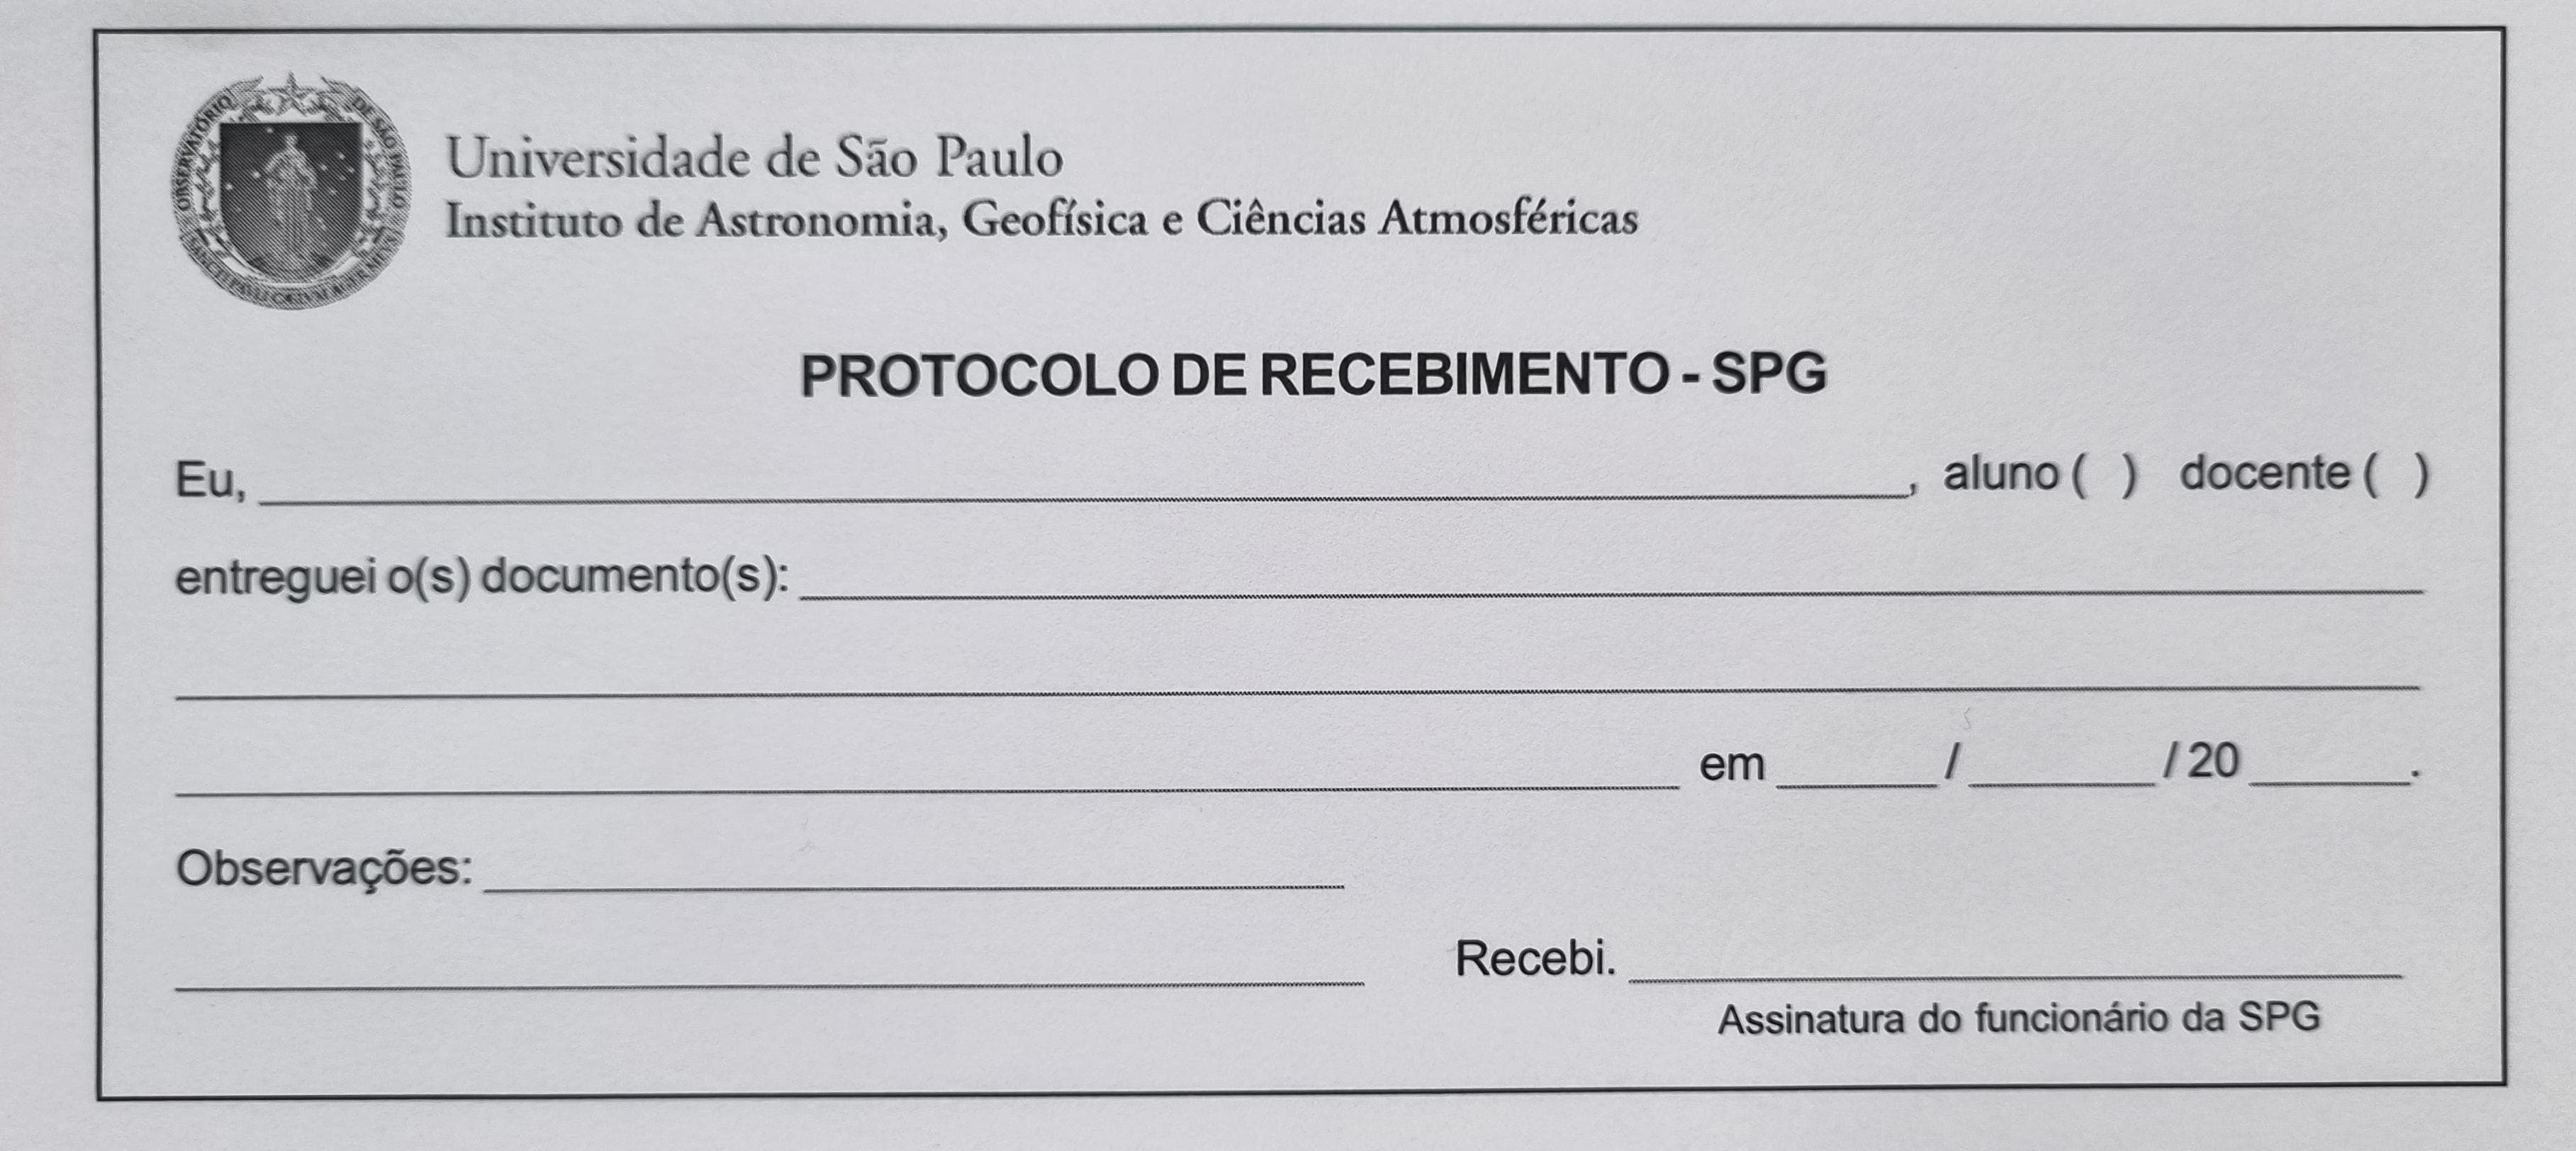
\includegraphics[width=\linewidth]{protocolo_recebimento.jpeg}
      \caption{Foto do protocolo de recebimento de depósito, que você precisa escanear e colocar no Janus.}
      \label{fig:protocolo}
    \end{figure}

    Para imprimir a tese, você pode aproveitar a parceria que o IAG tem com a gráfica do IME. Você só precisa mandar um email para a CCP (\url{ccpastro iag.usp.br}) pedindo autorização. Quando ela for dada, é só encaminhar o email para a Cida (\url{cida.coelho@iag.usp.br}), que fará a solicitação junto à grafica. Quando a impressão estiver pronta, depois de um ou dois dias, ela irá te avisar para você poder fazer a retirada. Note que talvez você tenha que falar com outra pessoa ao invés da Cida quando fizer a solicitação (este texto foi escrito em 2024).

    Tanto o formulário de sugestão da banca quanto a carta de manifestação do orientador estão disponíveis na seção de formulários do site do IAG (\url{https://www.iag.usp.br/pos-graduacao/formularios}), na parte ``8 - Defesa de Dissertações e Teses''. Para a sugestão da banca, a maioria dos examinadores deverá ser de fora do programa e pelo menos um de fora do IAG. Para o mestrado são necessários três titulares e três suplentes, enquanto que no doutorado são 5 titulares e 5 suplentes. Em ambos os casos você precisa colocar o nome do seu orientador(a) e um suplente correspondente. Recomendo você começar a conversar sobre os nomes um mês antes da data que você deseja fazer o depósito, assim você pode enviar emails para os examinadores perguntando se aceitam compor sua banca.

    Depois de entregar os documentos, a CCP irá julgar a sugestão para a banca e, caso aprovada, você terá até 105 dias para realizar a defesa. Caso queira defender em menos de 30 dias, é necessário preencher um termo de responsabilidade (também presente na parte de formulários do site do IAG).

  \section{Características deste template}
    Este template foi criado tendo como base o repositório Web\LaTeX{}, que por sua vez foi criado para substituir o Overleaf. A vantagem neste caso é a integração com o GitHub, permitindo o controle de versões, por exemplo, o uso de Codespaces (que são computadores virtuais, criados através do GitHub) caso você queira, e a possibilidade de usar extensões como Grammarly, LTex e Copilot. Caso você não queira usar um Codespace (pois ele é limitado a 180 horas de uso por mês), você também pode clonar o repositório pra o seu PC e trabalhar normalmente. Isso é possível pois o WebLaTex define um container com toda a informação necessária para você compilar seus documentos.

    \subsection{Web\LaTeX{}}
      O WebLaTex foi criado como uma alternativa de acesso aberto ao Overleaf, quando este começou a cobrar pelo serviço. Ele usa o VSCode como base e traz algumas extensões por padrão, como o GitHub Copilot, Grammarly, \LaTeX{} Workshop. Também existem algumas opcionais, como a Live Share, que permite que várias pessoas escrevam no mesmo arquivo simultaneamente (similar ao Overleaf).

      Da forma que ele está configurado neste template, o \LaTeX{} irá compilar o seu arquivo toda vez que você salvar, respeitando um intervalo mínimo de 15 segundos entre compilações. Você pode mudar isso nas opções, digitando ``auto build'' na busca e mudando os valores do ``Auto Build: Interval'' e do ``Auto Build: Run''.

      Você pode encontrar mais detalhes sobre Web\LaTeX{} no site do repositório: \url{https://github.com/sanjib-sen/WebLaTex}.

    \subsection{VSCode e suas extensões}
      Usando estes templates, você pode escrever seu texto usando o VSCode (ou o VSCodium). Este editor possui diversas opções de customização, desde a aparência até suas extensões.

      Na presente versão, o template habilita, além das extensões do WebLaTex, a extensão ``GitDoc''. Esta extensão faz commit+push automaticamente toda vez que você salva o arquivo ou em intervalos definidos pelo usuário. Você pode mudar as configurações do GitDoc indo nas opções e escrevendo ``gitdoc'' na busca. Por padrão, ele faz os commits e pushs a cada 30 segundos, caso existam mudanças.

    \subsection{Acrônimos}
      Para facilitar o gerenciamento de acrônimos, este template usa o pacote \ttt{acro}. Os acrônimos devem ser definidos previamente no arquivo ``Sections/0.2-list\_of\_acronyms.tex'', usando o seguinte formato:
      %
      \begin{lstlisting}[autogobble]
        \DeclareAcronym{acronym}{
          short = short name,
          long  = long name,
          cite  = citation %optional
        }
      \end{lstlisting}

      Desta forma, a primeira referência à um acrônimo é escrita normalmente, usando a forma ``longa'' e citando a referência, caso você tenha a definido. Por exemplo, o comando \ttt{\textbackslash ac\{splus\}} resultará em \ac{splus}.

      Se o acrônimo é usado apenas uma vez, como no caso anterior, ele não exibe a versão curta do nome. Caso você queira forçar que isso aconteça, mesmo que só use o acrônimo uma única vez, é só combinar o comando \ttt{\textbackslash ac\{vhs\}} com o \ttt{\textbackslash acuse\{vhs\}}. Por exemplo: \ac{vhs}\acuse{vhs}.

      Você também pode incluir texto usando o math-mode (\ttt{\textbackslash ac\{photoz\}}) \ac{photoz}. Você também pode usar o acrônimo no plural (\ttt{\textbackslash acp\{photoz\}}) \acp{photoz}, forçar o modo curto (\ttt{\textbackslash acs\{specz\}}) \acs{specz} ou longo (\ttt{\textbackslash acl\{specz\}}) \acl{specz}. Há também a possibilidade de colocar a primeira letra em maiúsculo (\ttt{\textbackslash Ac\{specz\}}) \Ac{specz}.

    \subsection{Citações}
      As citações são gerenciadas com o pacote \ttt{natbib}, e definidas no arquivo ``Sections/6-bibliography.tex'', no qual a lista com referências usadas é importada do arquivo ``Sections/reference\_list.bib''. 

      Este pacote suporta diferentes tipos de citações, todas descritas em detalhes aqui: \url{https://gking.harvard.edu/files/natnotes2.pdf}.

      Uma dica adicional para deixar o seu arquivo de referências bem organizado e bonito é usar o Bibtex Tidy (\url{https://flamingtempura.github.io/bibtex-tidy/index.html}), que alinha, ordena e arruma as citações.

    \subsection{Exemplos}
      Colocarei aqui alguns exemplos de imagens, tabelas, listings, equações e etc para facilitar a escrita do seu trabalho.

      \subsubsection{Imagens}
      Uma imagem centralizada no texto (Figura \ref{fig:ex_1col}):
      %
      \begin{figure}[h]
        \centering
        \includegraphics[width=0.5\linewidth]{example-image-a}
        \caption{Exemplo de imagem em uma coluna.}
        \label{fig:ex_1col}
      \end{figure}

      Duas imagens centralizadas no texto (Figura \ref{fig:sub_1} e \ref{fig:sub_2}, partes da Figura \ref{fig:ex_2cols}). Você pode fazer como neste exemplo, mas eu recomendo que faça isso direto no \ttt{Python} e coloque no \LaTeX{} como uma imagem só:
      %
      \begin{figure}[h]
        \centering
        \begin{subfigure}{.45\textwidth}
          \centering
          \includegraphics[width=0.8\linewidth]{example-image-a}
          \caption{Subfigura 1}
          \label{fig:sub_1}
        \end{subfigure}%
        \begin{subfigure}{.45\textwidth}
          \centering
          \includegraphics[width=0.8\linewidth]{example-image-b}
          \caption{Subfigura 2}
          \label{fig:sub_2}
        \end{subfigure}
        \caption{Uma imagem contendo duas subfiguras}
        \label{fig:ex_2cols}
      \end{figure}

      Para não numerar as figuras, é só colocar um asterisco no final do nome do ambiente (figure $\rightarrow$ figure*).
      
      \subsubsection{Tabelas}
        Este template usa o pacote \ttt{booktabs}, que permite fazer tabelas mais bonitas. Repare no uso do ``toprule'', ``midrule'', e ``bottomrule'':
        %
        \begin{table}[h!]
          \centering
          \caption{Exemplo de tabela.}
          \label{tab:ex_1}
          \begin{tabular}{ccc}
            \toprule
            \textbf{Coluna 1} & \textbf{Coluna 2} & \textbf{Coluna 3} \\ \midrule
            Célula 1          & Célula 2          & Célula 3          \\ 
            Célula 4          & Célula 5          & Célula 6          \\ 
            \bottomrule
          \end{tabular}
        \end{table}

        Caso queira tirar as ``sobras'' à esquerda e à direita, é só incluir um ``@\{\}'' antes e depois da configuração das colunas:
        %
        \begin{table}[h!]
          \centering
          \caption{Exemplo de tabela sem as margens.}
          \label{tab:ex_2}
          \begin{tabular}{@{}ccc@{}}
            \toprule
            \textbf{Coluna 1} & \textbf{Coluna 2} & \textbf{Coluna 3} \\ \midrule
            Célula 1          & Célula 2          & Célula 3          \\ 
            Célula 4          & Célula 5          & Célula 6          \\ 
            \bottomrule
          \end{tabular}
        \end{table}

        Outras opções para as colunas são \ttt{c} para centralizado, \ttt{l} para alinhado à esquerda, \ttt{r} para alinhado à direita, e \ttt{p\{X\}} para ter uma célula com tamanho fixo X (que pode ser dado em cm):
        %
        \begin{table}[h!]
          \centering
          \caption{Exemplo de tabela com tamanho fixo.}
          \label{tab:ex_3}
          \begin{tabular}{@{}lrp{5cm}@{}}
            \toprule
            \textbf{Coluna 1} & \textbf{Coluna 2} & \textbf{Coluna 3} \\ \midrule
            Célula 1          & Célula 2          & Célula 3          \\ 
            Célula 4          & Célula 5          & Célula 6          \\ 
            \bottomrule
          \end{tabular}
        \end{table}

        Você também pode criar células que abrangem várias linhas ou colunas usando os comandos \ttt{\textbackslash multirow\{número de linhas\}\{tamanho (ou * para automático)\}\{Texto\}} e \ttt{\textbackslash multicolumn\{número de colunas\}\{alinhamento (l, r, caption)\}\{Texto\}}:
        %
        \begin{table}[h!]
          \centering
          \caption{Exemplo de tabela com multirows e multicolumns.}
          \label{tab:ex_4}
          \begin{tabular}{@{}ccc@{}}
            \toprule
            \textbf{Coluna 1}             & \textbf{Coluna 2} & \textbf{Coluna 3} \\ \midrule
            \multirow{2}{*}{Célula 1 e 4} & \multicolumn{2}{c}{Células 2 e 3}     \\ 
                                          & Célula 5          & Célula 6          \\ 
            \bottomrule
          \end{tabular}
        \end{table}

        O template também inclui o pacote \ttt{threeparttable}, que permite colocar notas de rodapé em tabelas:
        %
        \begin{table}[h!]
          \centering
          \caption{Exemplo de tabela usando o \ttt{threeparttable}.}
          \label{tab:ex_5}
          \begin{threeparttable}
            \begin{tabular}{ccc}
              \toprule
              \textbf{Coluna 1} & \textbf{Coluna 2} & \textbf{Coluna 3} \\ \midrule
              Célula 1\tnote{a} & Célula 2          & Célula 3\tnote{c} \\ 
              Célula 4          & Célula 5\tnote{b} & Célula 6          \\ 
              \bottomrule
            \end{tabular}
            \begin{tablenotes}
              \item[a] Célula 1.
              \item[b] Célula 5.
              \item[c] Célula 3.
            \end{tablenotes}
          \end{threeparttable}
        \end{table}

        Para não numerar as tabelas, é só colocar um asterisco no final do nome do ambiente (table $\rightarrow$ table*).

      \subsubsection{Listings (códigos)}
        Para colocar códigos no texto, este template usa o pacote \ttt{listings} que, apesar de não ser tão completo quanto o \ttt{minted}, não usa o \ttt{Python} como requisito. Um exemplo de código geral foi dado acima, na forma de definir acrônimos:
        %
        \begin{lstlisting}[autogobble]
          \DeclareAcronym{acronym}{
            short = short name,
            long  = long name,
            cite  = citation %optional
          }
        \end{lstlisting}

        Porém você pode definir estilos (configurados no arquivo ``Sections/0.1-configurations.tex''). O estilo para Python já está definido (Código \ref{code}):
        %
        \begin{lstlisting}[label=code, language=Python, numbers=left, autogobble]
          class Nome():
          """
          Exemplo de classe para o template
      
          Args:
            ...
      
          Attributes:
            ...
      
          Methods:
            ...
      
          Returns:
            ...
          """
      
          def __init__(self, in_features, out_features):
              super().__init__()
              self.in_features = in_features
              self.out_features = out_features

          ...
        \end{lstlisting}

        Nos dois casos, o parâmetro ``autogobble'' serve para tirar espaços em branco extras. Não há como deixar o código sem numeração.

      \subsubsection{Equações}
        Equação simples, como a Equação \eqref{eq:drake}:
        %
        \begin{equation}
          N = R_* \cdot f_\text{P} \cdot n_e \cdot f_\text{l} \cdot f_\text{i} \cdot f_\text{c} \cdot L
          \label{eq:drake}
        \end{equation}

        Também é possível criar equações de várias linhas, com alinhamento (Equação \eqref{eq:aligned}):
        %
        \begin{align}
          y &= a \cdot x + b, \\
          k &= a \cdot x^2 + b \cdot x + c
          \label{eq:aligned}
        \end{align}

        E, por último, criar ``cases'' (Equação \eqref{eq:cases}). Só é necessário quebrar a linha dentro do ambiente \ttt{cases}:
        %
        \begin{align}
          x =
          \begin{cases}
            y,\text{ se } a > 0 \\
            z,\text{ se } a \leq 0
          \end{cases}
          \label{eq:cases}
        \end{align}

        Para não numerar as equações, é só colocar um asterisco no final do nome do ambiente (equation ou align $\rightarrow$ equation* ou align*).

      \subsection{Fazendo plots no \ttt{Matplotlib}}
        Para facilitar a vida, existe uma função que permite que você faça plots no \ttt{Matplotlib} com as dimensões exatas para colocar no seu texto, sem precisar mexer com as opções do \ttt{\textbackslash includegraphics}. A função é descrita em \url{https://jwalton.info/Embed-Publication-Matplotlib-Latex/}, e a função é:
        %
        \begin{lstlisting}[label=code, language=Python, numbers=left, autogobble]          
          def set_size(width, fraction=1, subplots=(1, 1)):
              """Set figure dimensions to avoid scaling in LaTeX.
          
              Parameters
              ----------
              width: float or string
                      Document width in points, or string of predined document type
              fraction: float, optional
                      Fraction of the width which you wish the figure to occupy
              subplots: array-like, optional
                      The number of rows and columns of subplots.
              Returns
              -------
              fig_dim: tuple
                      Dimensions of figure in inches
              """
              if width == 'thesis':
                  width_pt = 426.79135
              elif width == 'beamer':
                  width_pt = 307.28987
              else:
                  width_pt = width
          
              # Width of figure (in pts)
              fig_width_pt = width_pt * fraction
              # Convert from pt to inches
              inches_per_pt = 1 / 72.27
          
              # Golden ratio to set aesthetic figure height
              # https://disq.us/p/2940ij3
              golden_ratio = (5**.5 - 1) / 2
          
              # Figure width in inches
              fig_width_in = fig_width_pt * inches_per_pt
              # Figure height in inches
              fig_height_in = fig_width_in * golden_ratio * (subplots[0] / subplots[1])
          
              return (fig_width_in, fig_height_in)
        \end{lstlisting}

        Junto com essa definição, você deve configurar o \ttt{Matplotlib} pra usar estas configurações:
        %
        \begin{lstlisting}[label=code, language=Python, numbers=left, autogobble]          
          # Plot visual settings
          thesis_settings = {
              # Use LaTeX to write all text
              "text.usetex": False,
              "font.family": "serif",
              # Use 10pt font in plots, to match 10pt font in document
              "font.size": 10,
              "axes.labelsize": "medium",
              "axes.titlesize": "medium",
              "figure.labelsize": "medium",
              "figure.titlesize": "medium",
              # Make the legend/label fonts a little smaller
              "legend.fontsize": "small",
              "legend.title_fontsize": "small",
              "xtick.labelsize": "small",
              "ytick.labelsize": "small",
              # Enable axis grids
              "axes.grid": True,
              "grid.alpha": 0.5,
          }

          plt.rcParams.update(thesis_settings)
        \end{lstlisting}

        Feito isso, quando você for criar uma figura nova, é só chamar a função no argumento \ttt{figsize} usando \ttt{width = 455.24411} (que é a largura deste documento em pt). Por exemplo:
        \begin{lstlisting}[label=code, language=Python, numbers=left, autogobble]          
          fig, axes = plt.subplots(1, 2, figsize=set_size(width, suplots=(1, 2), fraction=1))
          ...
        \end{lstlisting}

        As outras opções e mais detalhes deste código estão descritas no link acima. Dois exemplos de imagens geradas com essa função estão nas Figuras \ref{fig:matplot_1} e \ref{fig:matplot_2}.
        %
        \begin{figure}[h]
          \centering
          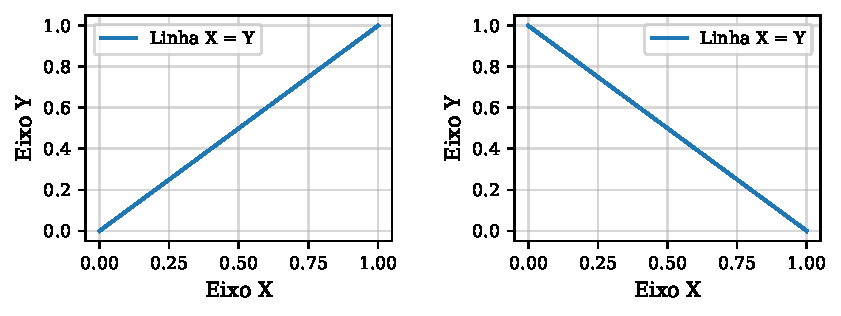
\includegraphics{exemplo_matplot_2.pdf}
          \caption{Exemplo de figura feita usando a função \ttt{set\_size}.}
          \label{fig:matplot_1}
        \end{figure}
        %
        \begin{figure}[h]
          \centering
          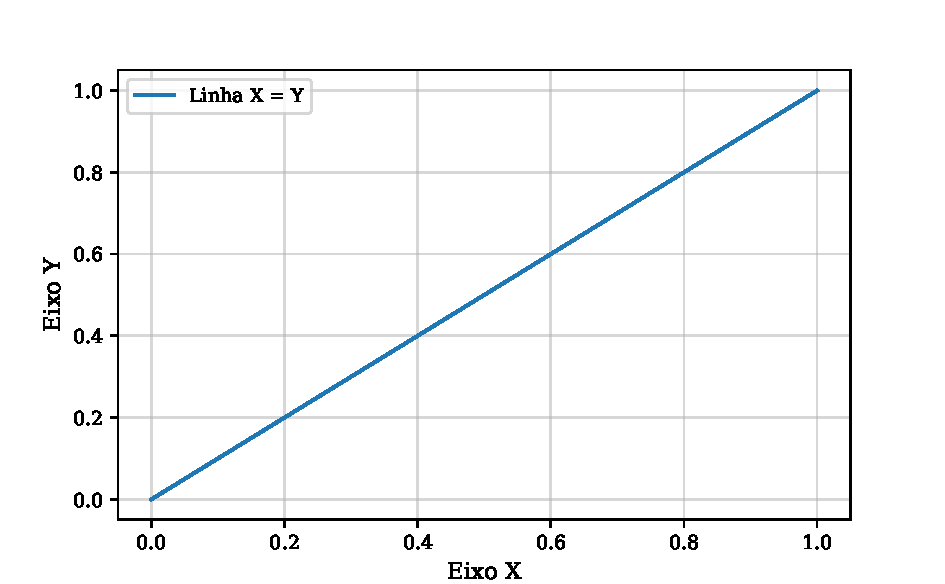
\includegraphics{exemplo_matplot.pdf}
          \caption{Exemplo de figura feita usando a função \ttt{set\_size}.}
          \label{fig:matplot_2}
        \end{figure}

        Note que nenhum caractere dentro da imagem tem tamanho menor do que os da legenda (que é um bom teste para saber se o tamanho das letras e números está bom) e como a imagem ocupa quase toda a largura do texto mesmo sem ser necessário usar a opção [width=\textbackslash linewidth].

      %     In this template, the citations are handled by the \ttt{natbib} package, with is defined by the commands in the ``Sections/6-bibliography.tex'' file. There, the list of used references are imported from the ``Sections/reference\_list.bib'' file.

  %     This package supports different types of citations, all of them explained here: \url{https://gking.harvard.edu/files/natnotes2.pdf}


  % The goal of this document is to provide an unofficial dissertation/thesis template for IAG/USP.

  % \section{General tips for when writing a dissertation/thesis}

  % When writing the text, you should be aware of the IAG/USP norms\footnote{\url{https://leginf.usp.br/?resolucao=resolucao-copgr-no-7882-de-25-de-novembro-de-2019}}. There are some obligatory chapters that should be in the text, the list is shown in ``XI – PROCEDIMENTOS PARA DEPÓSITO DA DISSERTAÇÃO/TESE''.

  % In order to make the deposit, you should have:
  % %
  % \begin{itemize}
  %   \item For PhD: a printed copy of the text, the forms containing the committee suggestion, a letter from the supervisor saying that you are fit for the defense, and proof of one published paper, where you are the first or second co-author, in a refereed international journal. You also need to make a deposit in Janus.
  %   \item For master's: 
  % \end{itemize}

  % IAG has a partnership with the IME's print shop. To print your dissertation/thesis with them you should send an email to \url{ccpastro iag.usp.br} with copy to \url{cida.coelho@iag.usp.br} asking for permission, with the PDF of the text attached. If approved, the text will be sent to the print shop and you will be notified when it is ready (within 1 or 2 days).

  % The forms for the committee and the supervisor manifestation can be found at IAG's website, in the ``Forms'' page: \url{https://www.iag.usp.br/pos-graduacao/formularios}. I recommend that you start thinking about the names that should be in your defense two weeks before making the deposit, and sending each member an email one week before, asking if they accept that their names be suggested.

  % \section{Features of this template}

  %   This template is based on the \ttt{WebLatex}\footnote{\url{https://github.com/sanjib-sen/WebLaTex}} template, created to replace Overleaf with Github, with some modifications. See the link for further details and the advantages of this approach.

  %   We also included the GitDoc extension, which automatically makes commit+push to a repository. To use it, you should enable the extension using \ttt{ctrl+shift+p} > ``GitDoc Enable''
  
  %   \subsection{Acronyms}
  %     The acronyms in this model are handled by the \ttt{acro} package, where you need to defined the acronyms beforehand, in the ``Sections/0.2-list\_of\_acronyms.tex'', using the format:

  %     \begin{lstlisting}[autogobble]
  %       \DeclareAcronym{acronym}{
  %         short = short name,
  %         long  = long name,
  %         cite  = citation %optional
  %       }
  %   \end{lstlisting}

  %   Using this package, the first reference to an acronym is written normally, with the reference if you defined the acronym with one, using the ``long'' name: \ac{splus}. Whenever you make another reference to this acronym, it will use the ``short'' name: \ac{splus}.
    
  %   You can also define acronyms using math-mode: \ac{photoz}. If you use the acronym only once, it will be printed using the long form only, without diplaying the short form, in this case, use can use the \ttt{\textbackslash ac\{acro\}} command followed by  \ttt{\textbackslash acuse\{acro\}}: \ac{specz}\acuse{specz}.

  %   There are some variations on how the acronyms can be printed, such as:
  %   \begin{itemize}
  %     \item Plural: \ttt{\textbackslash acp\{photoz\}} $\rightarrow$ \acp{photoz}
  %     \item Force long name: \ttt{\textbackslash acl\{des\}} $\rightarrow$ \acl{des}
  %     \item Force short name: \ttt{\textbackslash acs\{vhs\}} $\rightarrow$ \acs{vhs}
  %     \item Capital first letter: \ttt{\textbackslash Ac\{photoz\}} $\rightarrow$ \Ac{photoz}
  %   \end{itemize}

  %   \subsection{Citations}
  %     In this template, the citations are handled by the \ttt{natbib} package, with is defined by the commands in the ``Sections/6-bibliography.tex'' file. There, the list of used references are imported from the ``Sections/reference\_list.bib'' file.

  %     This package supports different types of citations, all of them explained here: \url{https://gking.harvard.edu/files/natnotes2.pdf}

  %   \subsection{Examples of tables, figures, listings...}

  %   \subsection{Making figures with \ttt{Matplotlib}}
\chapter{\chapternamemethodology}

\chapter{\chapternameresults}

\chapter{\chapternameconclusions}
  
\chapter{\chapternamefuture}
  
\newpage
\bibliographystyle{bib_style}
\bibliography{Sections/reference_list.bib}
\appendix
\chapter{\chapternameappendix}
    

\end{document}
